\subsection{Numerical Experiments}
Now that we've finally slogged through the presentation of the theory, we can
produce a few numerical experiments. Take, for example, the linear least squares
regression problem with $A \in \mathbb{R}^{n \times m}, x \in \mathbb{R}^m$ and
$b \in \mathbb{R}^n$:
\[
  f(x) = \frac{1}{2}\norm{Ax-b}_2^2 
  = \sum_{k=1}^n 
  \underbrace{ \frac{1}{2} (A_ix - b_i)^2 }_{f_i(x)}
\]
This is a particularily interesting example, as when we examing the stochastic
descent direction of this loss function:
\[
  \nabla f_i(x) = A_{i*}^T(A_{i*}x - b_i), 
  \text{ where }
  A = 
  \begin{bmatrix}
    A_{1*} \\
    \vdots \\
    A_{n*}
  \end{bmatrix}
\]
we notice that the sparsity pattern of $\nabla f_i(x)$ is entirely controlled by
by the sparsity pattern of the rows of $A$. This makes this problem
particularily convinient when trying to understand the effect of sparsity on the
asynchronous noise generated by \hogwild. The original paper \cite{2011NRRW}'s
results required strict assumptions on the sparsity pattern of $\nabla f_i(x)$
in order to guarantee convergence, but as we saw in Theorem
\ref{thm:convexconv}, as long as certain regularity properties are satisfied,
there's no need for such an assumption. Indeed $f$ does satisfy the above,
assuming that $A$ is of full rank%
\footnote{
  One subtle note is that the second condition is actually equivalent to having
  upper bounded maximal eigenvalue. I think we proved this back when we were
  discussing Nesterov's method, and also can be found at this stackexchange
  \url{https://math.stackexchange.com/a/1699082/245618}.
}. Therefore, when $A$ is both sparse and dense, we should see
a $\mathcal{O}(1/k)$ convergence rate, and indeed see figure
\ref{fig:convergence} for the validation of that.
\begin{figure}[!htb]
  \centering
  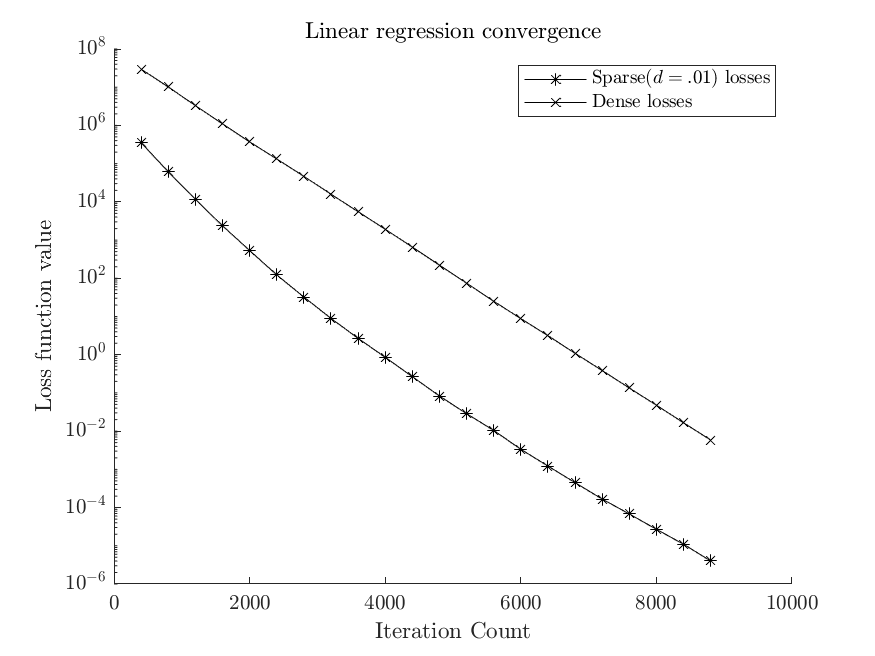
\includegraphics[width=.8\textwidth]{./resources/convergence}
  \caption{
    The matrix Sparse$(d = 0.1)$ is generated by the command {\tt
    sprand(n,m,.01)}. Playing with the density parameter doesn't change the
    shape of the convergence line, but note that denser matrices (since the
    entries are Gaussian) produce a higher initial loss and suffer from more
    asynchronous noise, and therefore require more iterations.
  } \label{fig:convergence}
\end{figure}

